\section{Evaluation}\label{sec:eval}

In this section, we first use a suite of microbenchmarks that target specific
operations (e.g., invoking a continuation, checkpointing, etc.) and orchestration
patterns (e.g., chaining, fan-out and fan-in) to understand unum's performance
characteristics and cost benefits.

We then evaluate unum's expressiveness and end-to-end performance with 6
real-world applications, taken from serverless application repositories and
research literature. Each application covers a different use case and
orchestration pattern.

We compare unum with the Step Functions Standard workflows. We do not include
Step Functions Express workflows in our evaluation because of its poor
execution guarantee: a single invocation could produce multiple different
answers.

We show that [Key results and takeaways in 3 sentences.]

\subsection{Experimental setup}

Lambda, 128MB memory size unless otherwise specified.

On-demand DynamoDB as the intermediary data store

Step Functions Standard

All experiments run in the same Region: us-west-1 (cali.)

We try to avoid function cold starts whenever we can by pre-warming the
functions before experiments. However, because of Lambda's concurrency limit,
it is difficult to eliminate eviction and cold starts for large-scale
workloads (e.g., ExCamera).

\subsection{Microbenchmarks}


\paragraph{How much additional latency does unum incur? How much does that
translate to costs?}

We first look at the performance and costs of the unum runtime. We measure the
latency of each primitive and the total additional latency for unum to take a
checkpoint and invoke a continuation. We translate the additional latency to
dollar costs in Lambda duration and compare it against Step Functions' costs
for state transitions. Note that unum taking a single checkpoint and invoking a
single continuation is equivalent to one Step Function state transition.

\begin{figure}[t!]
    \centering
    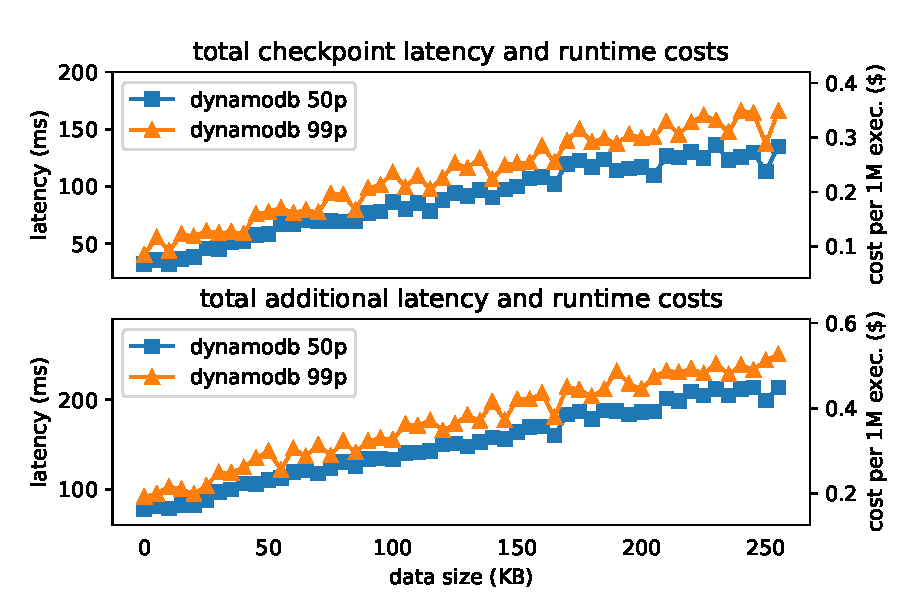
\includegraphics[width=\columnwidth]{figures/TotalAdditionalLatency.pdf}
    \caption{Total latency unum incurs for checkpointing and invoking a single
    continuation. We use a chain of two functions (\texttt{F->G}) that simply
    return their input. \texttt{data size} is the output data size of
    \texttt{F}, which in turn is the amount of data \texttt{F} writes to
    checkpoint and the input data size of \texttt{G}. We see that even at
    Lambda's payload size limit (256KB), unum's total runtime cost of
    checkpointing and invoking a continuation (50p: \$0.45 per 1M exec., 99p:
    \$0.53 per 1M exec.) is a mere fraction of Step Functions'
    cost of state transition (\$27.9 per 1M exec.). A Step Functions state
    transition is equivalent to unum checkpointing a function and invoking a
    single continuation.}
    \label{fig:totallatency}
\end{figure}

\begin{figure}[t!]
    \centering
    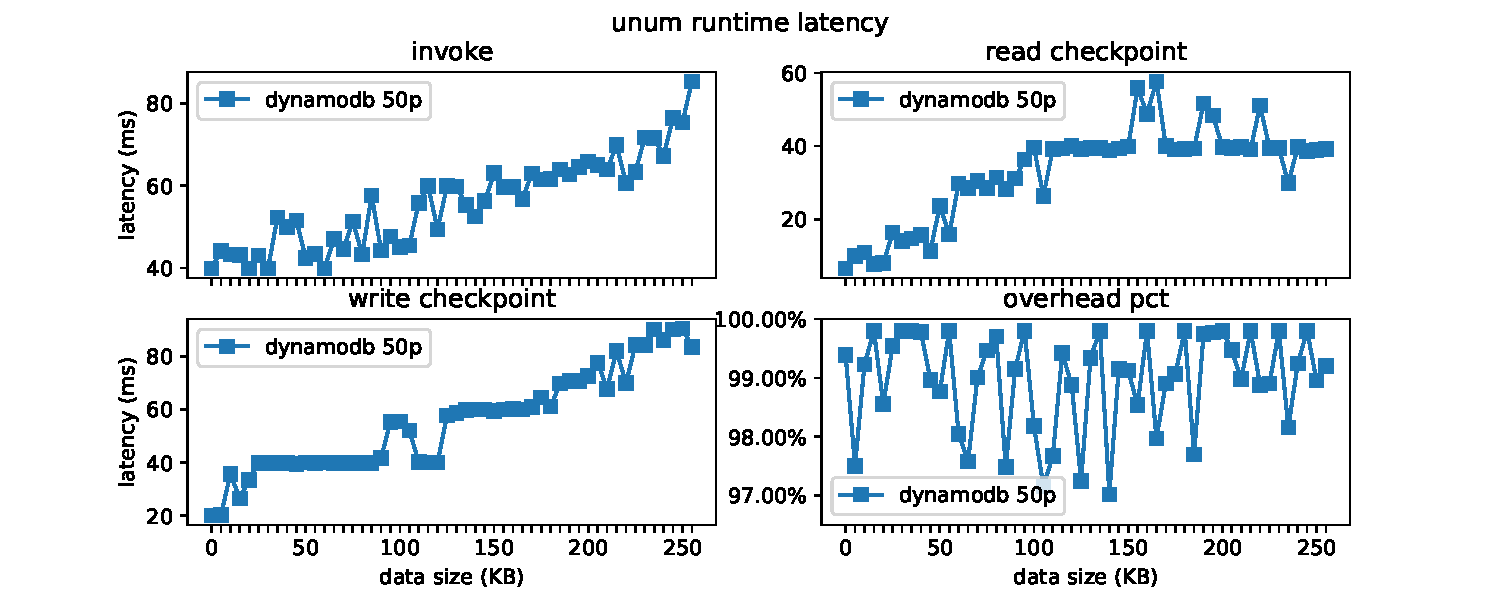
\includegraphics[width=\columnwidth]{figures/OpLatency.pdf}
    \caption{Average latency incured by unum primitives.}
    \label{fig:oplatency}
\end{figure}




\paragraph{How well does unum perform with orchestration primitives (chaining,
fan-out, fan-in)?}


Though we want to compare the performance of basic workflow operations (e.g.,
invoking a function, checkpointing) between unum and Step Functions, Step
Functions logs do not provide sufficiently granular timestamps for an
apple-to-apple comparison. Therefore, we instead measure the end-to-end
latency of buidling-block orchestration patterns -- chaining, fan-out and
fan-in. To make sure the measurements mostly reflect the performance of the
workflow system and not the latency of user code, we minimize function
duration to 1ms so that the majority of latency comes from the workflow
system.


\begin{figure}[t!]
    \centering
    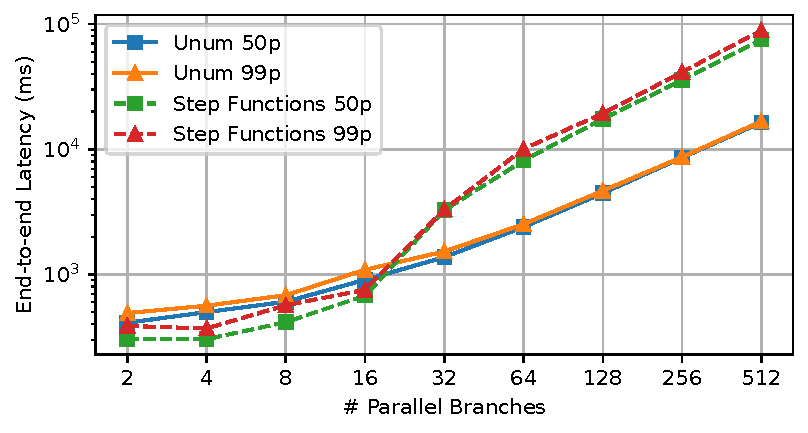
\includegraphics[width=\columnwidth]{figures/MapMicroLatency.pdf}
    \caption{End-to-end latency of parallel fan-out and fan-in. Lower is
    better. unum scales much better than the current version of Step Functions
    (experiments ran on Nov. 15, 2021) for parallel fan-out workloads. The
    result is not arguing that orchestrator-based workflow systems
    fundamentally scales worse than unum. In fact, the main cause of high
    latency in Step Functions is throttling of concurrent iterations when the
    fan-out size exceeds 40~\cite{aws-step-functions-map-state}. Although Step
    Functions does not elaborate on the reason for such throttling, there is
    little reason to believe that the maximum allowable concurrency is
    fundamentally capped around 40 for parallel workloads. However, this
    result does demonstrate an important downside of adding supplemental
    hosted services to support new workloads: any services added must also
    perform well compared with the highly scalable FaaS substrate and
    application developers must work with any restrictions that the services
    impose. unum avoids the additional work of building and maintaining hosted
    orchestrators and directly leverages the scalability of Lambda to achieve
    better parallel performance.}
    \label{fig:mapmicrolatency}
\end{figure}

\paragraph{What's the cost of checkpointing? The total cost of the equivalence
of a single Step Functions state transition.}




% \subsection{Key Results}

% Invocation latency and invocation latency vs input payload size.

% Invocation latency translate to price,, i.e., 1 million invocations = \$ vs Step Function each state transition.

% Checkpoint latency (including the first check if a checkpoint exists) and
% checkpoint latency vs input payload size up to the Lambda invocation payload
% size limit. Because if you write Lambda applications, once your data is larger
% than the input payload size, you'd do your own data management anyway. This is
% perhaps not ideal API but this is not something that unum changes. In fact,
% it's not clear whether we should change this because some types of data are
% better when used with a data store.

% Total, invocation latency + checkpoint latency vs input payload size and
% translate this to \$ and compare with Step Functions for for instance 1million
% invocations.

% Do the same for a fan-out and fan-in:

% The fan-out initiator is going to spend XX ms to invoke all fan-out functions.
% This number should be roughly linear to <fan-out size> * individual invocation
% latency. So the invocation latency for a single continuation should be
% sufficient.

% Each fan-out function needs to spend XX extra ms to write to DynamoDB and the
% last to finish is going to invoke the fan-in function.

% The fan-in function needs to spend XX extra ms to read from the intermediary
% data store.


% % -------------

% Chaining latency vs chain length, compare with Step Functions

% Map Latency vs map size, compare with Step Functions

%     Example of an artificial limitations on scalability with additional service approach

% % -------------

% real applications/macrobenchmarks or case study?

% Not sure how to present the results. All applications in the same table? or
% each application with its own subsection? What if we end up with some
% applications that deserve its own subsection and some don't? Answer: start by
% writing each application with its ownd subsection, pour everything out and
% then decide how to organize.



% % --------------

% (Not sure how to discuss the expressiveness advantage or whether we should
% discuss at all)

% Step Functions no way to express a for loop or fold.

% Step Functions no way to express pipeline parallelism.

% Step Functions fan-in needs to make sure the aggregate data doesn't exceed a
% limit, unum automatically passes data in using pointers to the intermediary
% data store.
\subsection{Macrobenchmarks}

\subsubsection{Applications}

% Non-contrived

% Representative

% Describe what each application does, What pattern they use, what 


% \begin{table}[]
% \begin{tabular}{llllll}
% \hline
%                      &                        & \multicolumn{2}{l}{\textbf{unum}}                                                                                                   & \multicolumn{2}{l}{\textbf{Step Functions}}                                                                     \\
% \textbf{Application} & Pattern                & \textit{e2e latency} & \textit{cost (per 1M exec.)}                                                                                 & \textit{e2e latency} & \textit{cost (per 1M exec.)}                                                             \\ \hline
% IoT Pipeline         & chain                  & 120.9ms              & $0.2*2+(73+28)*$0.0021+2*\$1.3942                                                                            & 226.52               & $0.2*2+ 4*$27.9                                                                          \\
% Text Processing      & fan-out, fan-in        & 562.69ms             & $0.2*6+ (105+149+70+68+144+100)*$0.0021 + 6*$1.3942+2*2*$0.279                                               & 552.46ms             & $0.2*5+7*$27.9                                                                           \\
% Wordcount            & chain, fan-out, fan-in & 410s                 & $0.2*(1+262+1+250+1) + (277+6264*262 + 348 + 667*250 +68)*$0.0021 +(1+262+1+250+1)*$1.3942 + 262*2*$0.279+ 250*2* $0.279    & 898s                 & $0.2*(1+262+1+250+1) + (5913*262 + 154 + 633*250 +5)*$0.0021 +(1+262+1+1+250+1+1)*\$27.9 \\
% ExCamera             & chain, fan-out, fold   & 84s                  & $0.2*(1+16+15+15+14) + (6500+1500+350+4500+5000)*$0.0021+ (1+16+15+15+14)*$1.3942 + 15*2*$0.279+14*2*\$0.279 & 98s                  & $0.2*(16+16+1+16+15)+(6300+1400+2+5500+5300)*$0.0021+(1+16+16+1+1+16+1+1)*\$27.9      \\ \hline
% \end{tabular}
% \end{table}

\begin{table*}[t]
\begin{tabular}{llllll}
\hline
                     &                        & \multicolumn{2}{c}{\textbf{unum}}                                                                                                   & \multicolumn{2}{c}{\textbf{Step Functions}}                                                                     \\
\textbf{Application} & \textbf{Pattern}                & \textit{e2e latency} & \textit{cost (per 1M exec.)}                                                                                 & \textit{e2e latency} & \textit{cost (per 1M exec.)}                                                             \\ \hline
IoT Pipeline         & chain                  & 120.9ms              & \$3.4005                                                                            & 226.52               & \$112                                                                          \\
Text Processing      & fan-out, fan-in        & 562.69ms             & \$12.0168                                               & 552.46ms             & \$196.3                                                                           \\
Wordcount            & chain, fan-out, fan-in & 410s                 & \$4904.79   & 898s                 & \$18113 \\
ExCamera             & chain, fan-out, fold   & 84s                  & \$150.91 & 98s                  & \$1530      \\ \hline
\end{tabular}
\end{table*}

\subsection{Writing Notes}

\subsubsection{What does success look like?}

\begin{enumerate}

    \item Expressiveness. That you can build a wide range of realistic
     applications with unum.

    \item Latency performance. That unum is on par with Step Functions.

    \item Cost. That running applications on unum is cheaper than Step
     Functions.

\end{enumerate}

We can tune the phrasing based on how much we promise in the Intro, but the
main metrics are the above three.

\subsubsection{Questions}

\begin{enumerate}

    \item How do we evaluate and present execution guarantee? Anything to show
     to convince our reader that it's correct?

    \item How do we evaluate other benefits that stem from a simpler design
     (the fact that unum gets rid of the needs for a separate orchestrator
     service), such as resource management, required staffing and other
     hosting costs.

    \item Should we run experiments with S3 and present those numbers?

\end{enumerate}


